%%%%%%%% ICML 2018 EXAMPLE LATEX SUBMISSION FILE %%%%%%%%%%%%%%%%%

\documentclass{article}

% Recommended, but optional, packages for figures and better typesetting:
\usepackage{microtype}
\usepackage{graphicx}
\usepackage{subfigure}
\usepackage{booktabs} % for professional tables

% added packages david
\usepackage{amsmath, amssymb}
\usepackage{bm}
\usepackage{subfigure}
\usepackage{tikz}


% hyperref makes hyperlinks in the resulting PDF.
% If your build breaks (sometimes temporarily if a hyperlink spans a page)
% please comment out the following usepackage line and replace
% \usepackage{icml2018} with \usepackage[nohyperref]{icml2018} above.
\usepackage{hyperref}

% Attempt to make hyperref and algorithmic work together better:
\newcommand{\theHalgorithm}{\arabic{algorithm}}

\newcommand\independent{\protect\mathpalette{\protect\independenT}{\perp}}
\def\independenT#1#2{\mathrel{\rlap{$#1#2$}\mkern2mu{#1#2}}}

% Use the following line for the initial blind version submitted for review:
%\usepackage{icml2018_ift6269}

% If accepted, instead use the following line for the camera-ready submission:
\usepackage[accepted]{icml2018_ift6269}
% SLJ: -> use this for your IFT 6269 project report!

% The \icmltitle you define below is probably too long as a header.
% Therefore, a short form for the running title is supplied here:
\icmltitlerunning{Submission and Formatting Instructions for ICML 2018}

\begin{document}

\twocolumn[
\icmltitle{Submission and Formatting Instructions for \\
           International Conference on Machine Learning (ICML 2018)}

% It is OKAY to include author information, even for blind
% submissions: the style file will automatically remove it for you
% unless you've provided the [accepted] option to the icml2018
% package.

% List of affiliations: The first argument should be a (short)
% identifier you will use later to specify author affiliations
% Academic affiliations should list Department, University, City, Region, Country
% Industry affiliations should list Company, City, Region, Country

% You can specify symbols, otherwise they are numbered in order.
% Ideally, you should not use this facility. Affiliations will be numbered
% in order of appearance and this is the preferred way.
\icmlsetsymbol{equal}{*}

\begin{icmlauthorlist}
\icmlauthor{Aeiau Zzzz}{equal,to}
\icmlauthor{Bauiu C.~Yyyy}{equal,to,goo}
\icmlauthor{Cieua Vvvvv}{goo}
\icmlauthor{Iaesut Saoeu}{ed}
\icmlauthor{Fiuea Rrrr}{to}
\icmlauthor{Tateu H.~Yasehe}{ed,to,goo}
\icmlauthor{Aaoeu Iasoh}{goo}
\icmlauthor{Buiui Eueu}{ed}
\icmlauthor{Aeuia Zzzz}{ed}
\icmlauthor{Bieea C.~Yyyy}{to,goo}
\icmlauthor{Teoau Xxxx}{ed}
\icmlauthor{Eee Pppp}{ed}
\end{icmlauthorlist}

\icmlaffiliation{to}{Department of Computation, University of Torontoland, Torontoland, Canada}
\icmlaffiliation{goo}{Googol ShallowMind, New London, Michigan, USA}
\icmlaffiliation{ed}{School of Computation, University of Edenborrow, Edenborrow, United Kingdom}

\icmlcorrespondingauthor{Cieua Vvvvv}{c.vvvvv@googol.com}
\icmlcorrespondingauthor{Eee Pppp}{ep@eden.co.uk}



% You may provide any keywords that you
% find helpful for describing your paper; these are used to populate
% the "keywords" metadata in the PDF but will not be shown in the document
\icmlkeywords{Machine Learning, ICML}

\vskip 0.3in
]

% this must go after the closing bracket ] following \twocolumn[ ...

% This command actually creates the footnote in the first column
% listing the affiliations and the copyright notice.
% The command takes one argument, which is text to display at the start of the footnote.
% The \icmlEqualContribution command is standard text for equal contribution.
% Remove it (just {}) if you do not need this facility.

%\printAffiliationsAndNotice{}  % leave blank if no need to mention equal contribution
\printAffiliationsAndNotice{\icmlEqualContribution} % otherwise use the standard text.

\begin{abstract}
This document provides a basic paper template and submission guidelines.
Abstracts must be a single paragraph, ideally between 4--6 sentences long.
Gross violations will trigger corrections at the camera-ready phase.
\end{abstract}

\section{Introduction}\label{sec:intro}

In recent years, deep learning has achieved remarkable success across a wide range of classification tasks, including image recognition, natural language processing, and medical diagnosis \cite{lecun2015deep}. Despite their high predictive accuracy, traditional neural networks often operate as black boxes, providing point estimates without quantifying the uncertainty associated with their predictions. This limitation poses significant challenges, especially in safety-critical applications such as autonomous driving, healthcare, and financial decision-making, where understanding the confidence of predictions is crucial for reliable and trustworthy outcomes \cite{kendall2017uncertainties}. Uncertainty estimation in neural networks addresses this challenge by providing measures of confidence alongside predictions. Bayesian Neural Networks (BNNs) offer a principled framework for uncertainty estimation by treating model parameters as random variables and capturing their posterior distribution \cite{blundell15}. By integrating over the uncertainty in the model parameters, BNNs can provide more robust predictions and better generalize to unseen data. However, exact Bayesian inference in neural networks is intractable due to the high dimensionality and complexity of the parameter space, necessitating the development of approximate inference methods. Several approaches have been proposed to approximate the posterior distribution in BNNs, each with its own set of advantages and limitations. Sampling-based methods like Stochastic Gradient Langevin Dynamics (SGLD) \cite{} and Hamiltonian Monte Carlo (HMC) \cite{neal12} provide accurate posterior approximations but are often computationally expensive and challenging to scale to large networks. On the other hand, approximation techniques such as Monte Carlo Dropout (MC Dropout) \cite{gal16} and Deep Ensembles \cite{lakshminarayanan17} offer more computationally feasible alternatives but may lack the theoretical rigor and flexibility to capture complex posterior distributions fully. Variational Inference (VI) methods, including Bayesian Backpropagation (BBP) \cite{blundell15}, strike a balance between scalability and accuracy but are constrained by the choice of variational families, which may oversimplify the true posterior. Despite these advancements, existing methods often face trade-offs between computational efficiency, scalability, and the fidelity of uncertainty estimates. In particular, many approaches rely on assumptions such as Gaussianity in the parameter or output space, which may not hold in practice, especially for complex and high-dimensional data distributions. Additionally, the computational overhead associated with sampling-based methods limits their applicability to large-scale classification tasks, prompting the need for more efficient inference techniques.

In this work, we implement a novel method that leverages Tractable Approximate Gaussian Inference (TAGI) to provide efficient and scalable uncertainty estimation in Bayesian Deep Networks. TAGI offers an to sampling-based approaches by maintaining and updating approximate Gaussian distributions over network parameters, enabling the propagation of uncertainty through deep learning models seamlessly. Furthermore, we propose a probabilistic softmax formulation that translates the uncertainty from the logit space to the output space, allowing for accurate and computationally efficient uncertainty estimates in classification tasks.

The focus of our project can be summarized as follows:

\begin{itemize}
    \item \textbf{Tractable Approximate Gaussian Inference (TAGI):} We re-implement the toy example proposed in the original TAGI paper \cite{goulet2020tractable}.
    \item \textbf{Probabilistic Softmax for Uncertainty Estimation:} We provide an implementation of the probabilistic softmax formulation porposed by the authors of TAGI, along with an evaluation on datasets such as MNIST and CIFAR-10.
    \item \textbf{Ablation Study:} We conduct an ablation study to evaluate the effectiveness of TAGI-based inference and the probabilistic softmax formulation in uncertainty estimation for classification tasks.
\end{itemize}

\section{Related Work}\label{sec:related_work}
Bayesian Neural Networks (BNNs) provide a principled framework for uncertainty estimation by capturing a posterior distribution over model parameters. Various methods, including sampling-based techniques and approximations, have been proposed to estimate uncertainty in classification tasks efficiently. Below, we review prominent methods alongside a recent advance using analytical approximations.

\subsection{Monte Carlo Dropout (MC Dropout)}
MC Dropout, introduced by \cite{gal16}, approximates Bayesian inference by using dropout during both training and inference. Multiple stochastic forward passes are performed at inference by sampling different dropout masks, and the outputs are aggregated to estimate the predictive distribution. The predictive mean is computed as:
$$
\hat{\mathbf{y}} = \frac{1}{T} \sum_{t=1}^{T} f(\mathbf{x}, \mathbf{w}^{(t)}),
$$
where  $\mathbf{w}^{(t)}$  are the sampled weights with dropout and  $T$  is the number of stochastic passes. This approach is computationally efficient and easy to implement but is limited by the reliance on dropout regularization, which might not fully capture posterior uncertainty.

\subsection{Stochastic Gradient Langevin Dynamics (SGLD)}
SGLD, proposed by \cite{well11}, combines stochastic gradient descent (SGD) with Langevin dynamics to sample from the posterior distribution of weights. The weight updates include Gaussian noise:
$$
\mathbf{w}_{t+1} = \mathbf{w}_t - \eta \nabla \mathcal{L}(\mathbf{w}_t) + \sqrt{2\eta} \epsilon_t,
$$
where  $\eta$  is the learning rate,  $\mathcal{L}$  is the loss function, and  $\epsilon_t \sim \mathcal{N}(0, I)$  is Gaussian noise. By incorporating noise into the gradient updates, SGLD provides samples that approximate the posterior. However, the method is more computationally intensive compared to approximation techniques like MC Dropout and can be sensitive to hyperparameters such as the step size.

\subsection{Hamiltonian Monte Carlo (HMC)}
HMC \cite{neal12} extends traditional Markov Chain Monte Carlo (MCMC) by using Hamiltonian dynamics to sample efficiently from the posterior. It introduces momentum variables and explores the posterior landscape using the Hamiltonian:
$$
\mathcal{H}(\mathbf{w}, \mathbf{p}) = -\log p(\mathbf{w} | \mathcal{D}) + \frac{\|\mathbf{p}\|^2}{2},
$$
where  $\mathbf{p}$  is the momentum. HMC provides accurate posterior samples, but its computational cost is prohibitive for high-dimensional neural network parameters. Additionally, it requires careful tuning of the step size and number of leapfrog steps.

\subsection{Bayesian Backpropagation (BBP)}
Bayesian Backpropagation (BBP), also known as Bayes by Backprop \cite{blundell15}, uses variational inference to approximate the posterior distribution over weights. A variational distribution  $q(\mathbf{w})$ , typically Gaussian, is optimized to minimize the Kullback-Leibler (KL) divergence from the true posterior. The variational posterior is parameterized as:
$$
q(\mathbf{w} | \boldsymbol{\theta}) = \prod_{i} \mathcal{N}(w_i; \mu_i, \sigma_i^2),
$$
where  $\boldsymbol{\theta} = (\boldsymbol{\mu}, \boldsymbol{\sigma})$  are learnable parameters. Inference involves sampling weights from  $q(\mathbf{w})$  and averaging multiple forward passes. While BBP provides a principled approach to Bayesian inference, the quality of the approximation depends on the chosen variational family, which might not fully capture the true posterior.

\subsection{Deep Ensembles}
Deep Ensembles \cite{NIPS2017} estimate uncertainty by training multiple neural networks with different random initializations. The ensemble predictions are averaged to compute the predictive distribution:
$$
\hat{\mathbf{y}} = \frac{1}{M} \sum_{m=1}^{M} f(\mathbf{x}; \mathbf{w}_m),
$$
where  $\mathbf{w}_m$  are the weights of the  $m^{th}$ ensemble member. The variance across the ensemble outputs represents model uncertainty. This method is robust and often outperforms other techniques in practice. However, it is computationally expensive due to the need to train multiple models independently.

\subsection{Variational Inference (VI)}
Variational Inference \cite{NIPS2011} approximates the posterior distribution  $p(\mathbf{w} | \mathcal{D})$  with a simpler variational distribution  $q(\mathbf{w})$  by minimizing the KL divergence:
$$
\text{KL}(q(\mathbf{w}) \| p(\mathbf{w} | \mathcal{D})) = \int q(\mathbf{w}) \log \frac{q(\mathbf{w})}{p(\mathbf{w} | \mathcal{D})} \, d\mathbf{w}.
$$
Common variational families include mean-field Gaussians, which are computationally efficient but may not fully capture the complexity of the true posterior. Variational inference is scalable and adaptable but often trades accuracy for efficiency.

\subsection{Fast Predictive Uncertainty for Classification with Bayesian Deep Networks}
\cite{hobbhahn22a} propose a method that revisits the Laplace Bridge technique to approximate the softmax output distribution using a Dirichlet distribution. The method maps Gaussian distributions in logit space  $\mathcal{N}(\mu, \Sigma)$  to Dirichlet distributions in output space  $\text{Dir}(\boldsymbol{\alpha})$  via the analytical mapping:
$$
\alpha_k = \exp\left(\mu_k + \frac{\sigma_k^2}{2}\right), \quad \text{for } k = 1, \ldots, K,
$$
where  $\mu_k$  and  $\sigma_k^2$  are the mean and variance of the logit for class  $k$ , and  $\alpha_k$  is the parameter of the resulting Dirichlet distribution. This approach avoids sampling and significantly reduces computational costs. It scales effectively to large datasets like ImageNet and complex architectures like DenseNet. While the method is efficient, its limitations include reliance on Gaussian assumptions in logit space and potential inaccuracies in modeling highly non-Gaussian posteriors. Additionally, its performance on small or imbalanced datasets is underexplored.

Each method offers unique strengths and weaknesses. MC Dropout and Deep Ensembles are practical and straightforward but may lack the theoretical rigor of sampling-based methods like SGLD and HMC. Variational inference approaches, such as BBP, balance scalability and accuracy but depend heavily on the choice of variational family. Sampling-based methods like SGLD and HMC provide accurate posterior approximations but are computationally expensive. The Dirichlet-based approach by Hobbhahn et al. introduces computational efficiency and scalability but trades off some flexibility in capturing complex posterior distributions.

In the next section, we introduce a novel method that combines the efficiency of analytical approximations with the theoretical grounding of Bayesian inference. The method relies on Tractable Approximate Gaussian Inference (TAGI) as a learning paradigm that allows passing uncertainty through deep learning models, and the formulation of a probabilistic softmax that further allows passing that uncertainty to the output layer.

\section{Methodology}\label{sec:methodology}
\subsection{Tractable approximate gaussian inference (TAGI)}\label{sub:tagi}
Goulet et al. \cite{goulet2020tractable} proposed the Tractable Approximate Gaussian Inference (TAGI) method, which is a Bayesian approach to neural networks. Compared to traditional NNs, this method allows to (1) optimize parameters analytically, (2) treat uncertainties from input to output layers and provide density forecasts. \\
Consider a fully connected NN presented in Figure \ref{fig:FNN},
the formulations of a TAGI-NN, which is similar to that of a traditional NN except that parameters and variables are assumed to be normally distributed, are defined by the following deterministic equations:
\begin{equation*} \label{eq:TAGI}
\begin{split}
    \bm{z}^{(1)} &= \bm{w}^{(0)} \bm{x} + \bm{b}^{(0)}, \\
    \bm{a}^{(i)} &= \tilde{\sigma}(\bm{z}^{(i)}) \; \; \;(i=1:\mathtt{L}), \\
    \bm{z}^{(i)} &= \bm{w}^{(i)} \bm{a}^{(i-1)} + \bm{b}^{(i)} \; \; \;(i=2:\mathtt{L}), \\
    \bm{z}^{(\mathtt{O})} &=  \bm{w}^{(\mathtt{L})} \bm{a}^{(\mathtt{L})} + \bm{w}^{(\mathtt{L})} \\
    \bm{y} &=  \bm{z}^{(\mathtt{O})} + \bm{v}.
\end{split}
\end{equation*}
where $\bm{w},\bm{b}$ are parameters, $\mathtt{L}$ is the number of hidden layers, $\bm{v}$ are the observation noise, $\bm{z}$ are hidden units, $\bm{y}$ are outputs, and $\tilde{\sigma}(\cdot)$ is the linearized activation function.
\begin{figure}[htbp]
\centering
\subfigure[]{\resizebox{0.9\linewidth}{!}{
\tikzset{dist1/.style={path picture= {
    \begin{scope}[x=1pt,y=10pt]
      \draw plot[domain=-6:6] (\x,{1/(1 + exp(-\x))-0.5});
    \end{scope}
    }
  }
}
\tikzset{dist2/.style={path picture= {
    \begin{scope}[x=1pt,y=10pt]
      \draw plot[domain=-6:6] (\x,{\x/10});
    \end{scope}
    }
  }
}
\tikzstyle{input}=[draw,fill=red!10,circle,minimum size=15pt,inner sep=0pt]
\tikzstyle{hidden}=[draw,fill=green!20,circle,minimum size=15pt,inner sep=0pt]
\tikzstyle{output}=[draw,fill=blue!20,circle,minimum size=15pt,inner sep=0pt]
\tikzstyle{bias}=[draw=none,circle,minimum size=15pt,inner sep=0pt]


\tikzstyle{stateTransition}=[->,line width=0.25pt,draw=black!50]


\begin{tikzpicture}[scale=1.36]\scriptsize
    \node (x1)[input]   at (0, 1.25) {$x_{1}$};
    \node (x2)[input] at (0, 0.25) {$x_{2}$};
    \node (x3)  at (0,-0.5) {\raisebox{6pt}{\vdots}};
    \node (xx)[input]  at (0,-1.25) {$x_{\mathtt{X}}$};

    \node (b0)[bias]  at (0.35,1.9) {$\bm{b}^{(0)}$};


    \node (h11)[hidden] at (1, 1.5) {$z^{(1)}_{1}$};
    \node (h12)[hidden] at (1, 0.5) {$z^{(1)}_{2}$};
    \node (h13) at (1,-0.5) {\raisebox{5pt}{$\vdots$}};
    \node (h14)[hidden] at (1,-1.5) {$z^{(1)}_{\mathtt{A}}$};
    \node (b1)[bias]  at (1.35,1.9) {$\bm{b}^{(1)}$};

    \node (h21)[hidden] at (2, 1.5) {$z^{(2)}_{1}$};
    \node (h22)[hidden] at (2, 0.5) {$z^{(2)}_{2}$};
    \node (h23) at (2,-0.5) {\raisebox{6pt}{\vdots}};
    \node (h24)[hidden] at (2,-1.5) {$z^{(2)}_{\mathtt{A}}$};
    \node (b2)[bias]  at (2.35,1.9) {$\bm{b}^{(\cdots)}$};
    
    \node (h31) at (3, 1.5) {$\cdots$};
    \node (h32) at (3, 0.5) {$\cdots$};
    \node (h33) at (3,-0.5) {\raisebox{6pt}{\vdots}};
    \node (h34) at (3,-1.5) {$\cdots$};
    \node (b3)[bias]  at (3.35,1.9) {$\bm{b}^{(\mathtt{L}-1)}$};
    
    \node (h41)[hidden] at (4, 1.5) {$z^{(\mathtt{L})}_{1}$};
    \node (h42)[hidden] at (4, 0.5) {$z^{(\mathtt{L})}_{2}$};
    \node (h43) at (4,-0.5) {\raisebox{6pt}{\vdots}};
    \node (h44)[hidden] at (4,-1.5) {$z^{(\mathtt{L})}_{\mathtt{A}}$};
    \node (b4)[bias]  at (4.35,1.9) {$\bm{b}^{(\mathtt{L})}$};

    \node (h1)[hidden] at (5.1,1.25) {$z_{1}^{(\mathtt{O})}$};
    \node (h2)[hidden] at (5.1,0.25) {$z_{2}^{(\mathtt{O})}$};
    \node (hn) at (5.1,-0.5) {\raisebox{6pt}{\vdots}};
    \node (h3)[hidden] at (5.1,-1.25) {$z_{\mathtt{Y}}^{(\mathtt{O})}$};
    \node (o1)[output] at (5.7,1.25) {$y_{1}$};
    \node (o2)[output] at (5.7,0.25) {$y_{2}$};
    \node (on) at (5.7,-0.5) {\raisebox{6pt}{\vdots}};
    \node (o3)[output] at (5.7,-1.25) {$y_{\mathtt{Y}}$};
    

    \draw[stateTransition] (x1) -- (h11) node  {};
    \draw[stateTransition] (x1) -- (h12) node  {};
    \draw[stateTransition] (x1) -- (h13) node  {};
    \draw[stateTransition] (x1) -- (h14) node  {};
    \draw[stateTransition] (x2) -- (h11) node  {};
    \draw[stateTransition] (x2) -- (h12) node  {};
    \draw[stateTransition] (x2) -- (h13) node  {};
    \draw[stateTransition] (x2) -- (h14) node  {};
    \draw[stateTransition] (x3) -- (h11) node  {};
    \draw[stateTransition] (x3) -- (h12) node  {};
    \draw[stateTransition] (x3) -- (h13) node  {};
    \draw[stateTransition] (x3) -- (h11) node  {};
    \draw[stateTransition] (xx) -- (h11) node  {};
    \draw[stateTransition] (xx) -- (h12) node  {};
    \draw[stateTransition] (xx) -- (h13) node  {};
    \draw[stateTransition] (xx) -- (h11) node  {};
     \draw[stateTransition] (xx) -- (h14) node  {};
    
    \draw[stateTransition] (b0) -- (h12) node {};
    \draw[stateTransition] (b0) -- (h11) node {};
    \draw[stateTransition] (b0) -- (h13) node {};
    \draw[stateTransition] (b0) -- (h14) node {};

    \draw[stateTransition,opacity=1] (h11) -- (h21) node [midway, rotate=0,fill=white,opacity=0.8] {\scriptsize$w^{(1)}_{1,1}$};
    \draw[stateTransition,opacity=0] (h11) -- (h21) node [midway, rotate=0,fill=white] {\scriptsize$w^{(1)}_{1,1}$};
    \draw[stateTransition,opacity=0.2] (h11) -- (h22) node  {};
    \draw[stateTransition,opacity=0.2] (h11) -- (h23) node  {};
    \draw[stateTransition,opacity=0.2] (h11) -- (h24) node  {};
    \draw[stateTransition,opacity=1] (h12) -- (h21) node [midway, rotate=45,fill=white,opacity=0.8] {\scriptsize$w^{(1)}_{1,2}$};
        \draw[stateTransition,opacity=0] (h12) -- (h21) node [midway, rotate=45,fill=white!90] {\scriptsize$w^{(1)}_{2,1}$};
    \draw[stateTransition,opacity=0.2] (h12) -- (h22) node  {};
    \draw[stateTransition,opacity=0.2] (h12) -- (h23) node  {};
    \draw[stateTransition,opacity=0.2] (h12) -- (h24) node  {};
    %\draw[stateTransition,opacity=0.2] (h13) -- (h21) node  {};
        \draw[stateTransition,opacity=1] (h13) -- (h21) node [midway, rotate=60,fill=white,opacity=0.8] {\scriptsize$w^{(1)}_{1,i}$};
     \draw[stateTransition,opacity=0] (h13) -- (h21) node [midway, rotate=60] {\scriptsize$w^{(1)}_{i,1}$};
    \draw[stateTransition,opacity=0.2] (h13) -- (h22) node  {};
    \draw[stateTransition,opacity=0.2] (h13) -- (h23) node  {};
    \draw[stateTransition,opacity=0.2] (h13) -- (h24) node  {};
    \draw[stateTransition,opacity=1] (h14) -- (h21) node [midway, rotate=70,fill=white,opacity=0.8] {\scriptsize$w^{(1)}_{1,\mathtt{A}}$};
     \draw[stateTransition,opacity=0] (h14) -- (h21) node [midway, rotate=70] {\scriptsize$w^{(1)}_{\mathtt{A},1}$};
    \draw[stateTransition,opacity=0.2] (h14) -- (h22) node  {};
    \draw[stateTransition,opacity=0.2] (h14) -- (h23) node  {};
    \draw[stateTransition,opacity=0.2] (h14) -- (h24) node  {};

    
    \draw[stateTransition,opacity=1] (b1) -- (h21) node  [midway,above=-0.05cm, rotate=-25] {\scriptsize$b^{(1)}_{1}$};
    \draw[stateTransition,opacity=0.2] (b1) -- (h22) node {};
    \draw[stateTransition,opacity=0.2] (b1) -- (h23) node {};
    \draw[stateTransition,opacity=0.2] (b1) -- (h24) node {};
    
     \draw[stateTransition] (h21) -- (h31) node  {};
    \draw[stateTransition] (h21) -- (h32) node  {};
    \draw[stateTransition] (h21) -- (h33) node  {};
    \draw[stateTransition] (h21) -- (h34) node  {};
    \draw[stateTransition] (h22) -- (h31) node  {};
    \draw[stateTransition] (h22) -- (h32) node  {};
    \draw[stateTransition] (h22) -- (h33) node  {};
    \draw[stateTransition] (h22) -- (h34) node  {};
    \draw[stateTransition] (h23) -- (h31) node  {};
    \draw[stateTransition] (h23) -- (h32) node  {};
    \draw[stateTransition] (h23) -- (h33) node  {};
    \draw[stateTransition] (h23) -- (h34) node  {};
    \draw[stateTransition] (h24) -- (h31) node  {};
    \draw[stateTransition] (h24) -- (h32) node  {};
    \draw[stateTransition] (h24) -- (h33) node  {};
    \draw[stateTransition] (h24) -- (h31) node  {};
    \draw[stateTransition] (h24) -- (h34) node  {};

    
    \draw[stateTransition] (b2) -- (h32) node {};
    \draw[stateTransition] (b2) -- (h31) node {};
    \draw[stateTransition] (b2) -- (h33) node {};
    \draw[stateTransition] (b2) -- (h34) node {};
    
    \draw[stateTransition] (h31) -- (h41) node  {};
    \draw[stateTransition] (h31) -- (h42) node  {};
    \draw[stateTransition] (h31) -- (h43) node  {};
    \draw[stateTransition] (h31) -- (h44) node  {};
    \draw[stateTransition] (h32) -- (h41) node  {};
    \draw[stateTransition] (h32) -- (h42) node  {};
    \draw[stateTransition] (h32) -- (h43) node  {};
    \draw[stateTransition] (h32) -- (h44) node  {};
    \draw[stateTransition] (h33) -- (h41) node  {};
    \draw[stateTransition] (h33) -- (h42) node  {};
    \draw[stateTransition] (h33) -- (h43) node  {};
    \draw[stateTransition] (h33) -- (h44) node  {};
    \draw[stateTransition] (h34) -- (h41) node  {};
    \draw[stateTransition] (h34) -- (h42) node  {};
    \draw[stateTransition] (h34) -- (h43) node  {};
    \draw[stateTransition] (h34) -- (h41) node  {};
     \draw[stateTransition] (h34) -- (h44) node  {};
    
    \draw[stateTransition] (b3) -- (h42) node {};
    \draw[stateTransition] (b3) -- (h41) node {};
    \draw[stateTransition] (b3) -- (h43) node {};
    \draw[stateTransition] (b3) -- (h44) node {};
    
    
    \draw[stateTransition] (h41) -- (h1) node  {};
    \draw[stateTransition] (h42) -- (h1) node  {};
    \draw[stateTransition] (h43) -- (h1) node  {};
    \draw[stateTransition] (h44) -- (h1) node  {};
    \draw[stateTransition] (b4) -- (h1) node {};
    
    \draw[stateTransition] (h41) -- (h2) node  {};
    \draw[stateTransition] (h42) -- (h2) node  {};
    \draw[stateTransition] (h43) -- (h2) node  {};
    \draw[stateTransition] (h44) -- (h2) node  {};
    \draw[stateTransition] (b4) -- (h2) node {};
    
    \draw[stateTransition] (h41) -- (hn) node  {};
    \draw[stateTransition] (h42) -- (hn) node  {};
    \draw[stateTransition] (h43) -- (hn) node  {};
    \draw[stateTransition] (h44) -- (hn) node  {};
    \draw[stateTransition] (b4) -- (hn) node {};
    
    \draw[stateTransition] (h41) -- (h3) node  {};
    \draw[stateTransition] (h42) -- (h3) node  {};
    \draw[stateTransition] (h43) -- (h3) node  {};
    \draw[stateTransition] (h44) -- (h3) node  {};
    \draw[stateTransition] (b4) -- (h3) node {};
    
     \draw[stateTransition] (h1) -- (o1) node  {};
     \draw[stateTransition] (h2) -- (o2) node  {};
     \draw[stateTransition] (hn) -- (on) node  {};
     \draw[stateTransition] (h3) -- (o3) node  {};
     
     \node (h12)[hidden] at (1, 0.5) {$z^{(1)}_{2}$};
     \node (h22)[hidden] at (2, 0.5) {$z^{(2)}_{2}$};

\end{tikzpicture}
}}\\
\subfigure[]{\resizebox{0.9
\linewidth}{!}{
\tikzset{dist1/.style={path picture= {
    \begin{scope}[x=1pt,y=10pt]
      \draw plot[domain=-6:6] (\x,{1/(1 + exp(-\x))-0.5});
    \end{scope}
    }
  }
}
\tikzset{dist2/.style={path picture= {
    \begin{scope}[x=1pt,y=10pt]
      \draw plot[domain=-6:6] (\x,{\x/10});
    \end{scope}
    }
  }
}
\tikzstyle{input}=[draw,fill=red!10,circle,minimum size=15pt,inner sep=0pt]
\tikzstyle{hidden}=[draw,fill=green!20,circle,minimum size=15pt,inner sep=0pt]
\tikzstyle{output}=[draw,fill=blue!20,circle,minimum size=15pt,inner sep=0pt]
\tikzstyle{bias}=[draw=none,circle,minimum size=15pt,inner sep=0pt]


\tikzstyle{stateTransition}=[->,line width=0.25pt,draw=black!50]


\begin{tikzpicture}[scale=1.36]\scriptsize
    \node (x)[input]   at (0, 1.5) {$\bm{x}$};
    \node (z1)[hidden] at (1, 1.5) {$\,\bm{z}^{(1)}$};
    \node (z2)[hidden] at (2, 1.5) {$\,\bm{z}^{(2)}$};
    \node (zi) at (3, 1.5) {$\cdots$};
    \node (zL)[hidden] at (4, 1.5) {$\,\bm{z}^{(\mathtt{L})}$};
    \node (zO)[hidden] at (5.1,1.5) {$\,\bm{z}^{(\mathtt{O})}$};
        %\node (zO)[hidden,fill=cyan!20] at (5.1,1.5) {$\,\bm{z}^{\!(\mathtt{O})}$};

    \node (y)[output] at (5.7,1.5) {$\bm{y}$};
   
   
    \draw[stateTransition,opacity=1] (x) -- (z1) node [midway, rotate=0,fill=white,opacity=0.8] {\scriptsize$\!\bm{\theta}^{(0)}\!$};
    \draw[stateTransition,opacity=1] (z1) -- (z2) node [midway, rotate=0,fill=white,opacity=0.8] {\scriptsize$\!\bm{\theta}^{(1)}\!$};
     \draw[stateTransition,opacity=1] (z2) -- (zi) node [midway, rotate=0,fill=white,opacity=0.8] {\scriptsize$\!\bm{\theta}^{(2)}\!$};
     \draw[stateTransition,opacity=1] (zi) -- (zL) node [midway, rotate=0,fill=white,opacity=0.8] {\scriptsize$\!\!\bm{\theta}^{(\mathtt{L}\text{-}1)}\!\!$};
    \draw[stateTransition,opacity=1] (zL) -- (zO) node [midway, rotate=0,fill=white,opacity=0.8] {\scriptsize$\!\bm{\theta}^{(\mathtt{L})}\!$};
     \draw[stateTransition,opacity=1] (zO) -- (y);
\end{tikzpicture}
}}
\caption{(a) A neural network representation. (b) A compacted NN representation, reproduced from \cite{goulet2020tractable}.}
\label{fig:FNN}
\end{figure}

In Equation \ref{eq:TAGI}, the product of two Gaussian random variables is not Gaussian, despite of this, the authors proposed using the \textit{Gaussian Multiplication Approximation} (GMA) to approximate the PDF of any product term $X_iX_j$ given by
%

% First Equation
\begin{equation*}
    \mathbb{E}\left[X_{1} X_{2}\right] = \mu_{1} \mu_{2} + \operatorname{cov}\left(X_{1}, X_{2}\right)
\end{equation*}
% Second Equation
\begin{equation*}
    \operatorname{cov}\left(X_{3}, X_{1} X_{2}\right) = \operatorname{cov}\left(X_{1}, X_{3}\right) \mu_{2} + \operatorname{cov}\left(X_{2}, X_{3}\right) \mu_{1}
\end{equation*}
% Third Equation - Split into Multiple Lines
\begin{align*}
    \operatorname{cov}\left(X_{1} X_{2}, X_{3} X_{4}\right) &= \operatorname{cov}\left(X_{1}, X_{3}\right) \operatorname{cov}\left(X_{2}, X_{4}\right) \nonumber \\
    &\quad + \operatorname{cov}\left(X_{1}, X_{4}\right) \operatorname{cov}\left(X_{2}, X_{3}\right) \nonumber \\
    &\quad + \operatorname{cov}\left(X_{1}, X_{3}\right) \mu_{2} \mu_{4} \nonumber \\
    &\quad + \operatorname{cov}\left(X_{1}, X_{4}\right) \mu_{2} \mu_{3} \nonumber \\
    &\quad + \operatorname{cov}\left(X_{2}, X_{3}\right) \mu_{1} \mu_{4} \nonumber \\
    &\quad + \operatorname{cov}\left(X_{2}, X_{4}\right) \mu_{1} \mu_{3}
\end{align*}
% Fourth Equation - Split into Multiple Lines
\begin{align*}
    \operatorname{var}\left(X_{1} X_{2}\right) &= \sigma_{1}^{2} \sigma_{2}^{2} + \operatorname{cov}\left(X_{1}, X_{2}\right)^{2} \nonumber \\
    &\quad + 2 \operatorname{cov}\left(X_{1}, X_{2}\right) \mu_{1} \mu_{2} \nonumber \\
    &\quad + \sigma_{1}^{2} \mu_{2}^{2} + \sigma_{2}^{2} \mu_{1}^{2}
\end{align*}
where $\mu, \sigma$ are respectively the mean and standard deviation of a random variable. 
Unlike a traditional NN where parameters are updated using backpropagation, model parameters in a TAGI-NN can be obtained analytically by a layer-wise scheme as depicted in Figure \ref{fig:updateTAGI}.
\begin{figure}[htbp]
\centering
\resizebox{0.9\linewidth}{!}{
\tikzset{dist1/.style={path picture= {
    \begin{scope}[x=1pt,y=10pt]
      \draw plot[domain=-6:6] (\x,{1/(1 + exp(-\x))-0.5});
    \end{scope}
    }
  }
}
\tikzset{dist2/.style={path picture= {
    \begin{scope}[x=1pt,y=10pt]
      \draw plot[domain=-6:6] (\x,{\x/10});
    \end{scope}
    }
  }
}
\tikzstyle{input}=[draw,fill=red!10,circle,minimum size=15pt,inner sep=0pt]
\tikzstyle{hidden}=[draw,fill=green!20,circle,minimum size=15pt,inner sep=0pt]
\tikzstyle{output}=[draw,fill=blue!20,circle,minimum size=15pt,inner sep=0pt]
\tikzstyle{bias}=[draw=none,circle,minimum size=15pt,inner sep=0pt]


\tikzstyle{stateTransition}=[->,line width=0.25pt,draw=black!50]


\begin{tikzpicture}[scale=1.36]\scriptsize
    \node (x)[input]   at (0, 1.5) {$\bm{x}$};
    \node (z1)[hidden] at (1, 1.5) {$\,\bm{z}^{(1)}$};
    \node (z2)[hidden] at (2, 1.5) {$\,\bm{z}^{(2)}$};
    \node (zi) at (3, 1.5) {$\cdots$};
    \node (zL)[hidden] at (4, 1.5) {$\,\bm{z}^{(\mathtt{L})}$};
    \node (zO)[hidden] at (5.1,1.5) {$\,\bm{z}^{(\mathtt{O})}$};
        %\node (zO)[hidden,fill=cyan!20] at (5.1,1.5) {$\,\bm{z}^{\!(\mathtt{O})}$};

    \node (y)[output] at (5.7,1.5) {$\bm{y}$};
   
   
    \draw[stateTransition,opacity=1] (x) -- (z1) node [midway, rotate=0,fill=white,opacity=0.8] {\scriptsize$\!\bm{\theta}^{(0)}\!$};
    \draw[stateTransition,opacity=1] (z1) -- (z2) node [midway, rotate=0,fill=white,opacity=0.8] {\scriptsize$\!\bm{\theta}^{(1)}\!$};
     \draw[stateTransition,opacity=1] (z2) -- (zi) node [midway, rotate=0,fill=white,opacity=0.8] {\scriptsize$\!\bm{\theta}^{(2)}\!$};
     \draw[stateTransition,opacity=1] (zi) -- (zL) node [midway, rotate=0,fill=white,opacity=0.8] {\scriptsize$\!\!\bm{\theta}^{(\mathtt{L}\text{-}1)}\!\!$};
    \draw[stateTransition,opacity=1] (zL) -- (zO) node [midway, rotate=0,fill=white,opacity=0.8] {\scriptsize$\!\bm{\theta}^{(\mathtt{L})}\!$};
     \draw[stateTransition,opacity=1] (zO) -- (y);
     
     \path (y) edge [->, cyan, opacity=0.8, bend left] (zO);
     \path (zO) edge [->, cyan, opacity=0.8, bend left] (zL);
     \path (zO) edge [->, cyan, opacity=0.8, bend left] (4.5,1.45);
     \path (zL) edge [->, cyan, opacity=0.8, bend left] (3,1.45);
     \path (zL) edge [->, cyan, opacity=0.8, bend left] (3.5,1.45);
     \path (zi) edge [->, cyan, opacity=0.8, bend left] (z2);
     \path (zi) edge [->, cyan, opacity=0.8, bend left] (2.5,1.45);
     \path (z2) edge [->, cyan, opacity=0.8, bend left] (z1);
     \path (z2) edge [->, cyan, opacity=0.8, bend left] (1.5,1.45);
     \path (z1) edge [->, cyan, opacity=0.8, bend left] (.5,1.45);
     
\end{tikzpicture}
}
\caption{Recursive layer-wise inference, reproduced from \cite{goulet2020tractable}.  Cyan arrows indicate inference directions.}
\label{fig:updateTAGI}
\end{figure}
%
First, given the observations $\bm{y}$, the output layer is updated as
\begin{equation*} \label{eq:z0update}
\begin{aligned}
f\left(\boldsymbol{z}^{(\mathtt{O})} \mid \boldsymbol{y}\right) &=\mathcal{N}\left(\boldsymbol{z}^{(\mathtt{O})} ; \boldsymbol{\mu}_{\boldsymbol{Z}^{(\mathtt{O})} \mid \boldsymbol{y}}, \boldsymbol{\Sigma}_{\boldsymbol{Z}^{(\mathtt{O})} \mid \boldsymbol{y}}\right) \\
\boldsymbol{\mu}_{\boldsymbol{Z}^{(\mathtt{O})} \mid \boldsymbol{y}} &=\boldsymbol{\mu}_{\boldsymbol{Z}^{(\mathtt{O})}}+\boldsymbol{\Sigma}_{\boldsymbol{Y} \boldsymbol{Z}^{(\mathtt{O})}}^{\top} \boldsymbol{\Sigma}_{\boldsymbol{Y}}^{-1}\left(\boldsymbol{y}-\boldsymbol{\mu}_{\boldsymbol{Y}}\right) \\
\boldsymbol{\Sigma}_{\boldsymbol{Z}^{(\mathtt{O})} \mid \boldsymbol{y}} &=\boldsymbol{\Sigma}_{\boldsymbol{Z}^{(\mathtt{O})}}-\boldsymbol{\Sigma}_{\boldsymbol{Y} \boldsymbol{Z}^{(\mathtt{O})}}^{\top} \boldsymbol{\Sigma}_{\boldsymbol{Y}}^{-1} \boldsymbol{\Sigma}_{\boldsymbol{Y Z}^{(\mathtt{O})}}.
\end{aligned}
\end{equation*}
%
Next, the hidden units and parameters of the layer $i^{th}$ are updated using a layer-wise procedure as
\begin{equation*}  \label{eq:layerwiseupdate}
\begin{aligned}
f(\boldsymbol{z} \mid \boldsymbol{y}) &=\mathcal{N}\left(\boldsymbol{z} ; \boldsymbol{\mu}_{\boldsymbol{Z} \mid \boldsymbol{y}}, \boldsymbol{\Sigma}_{\boldsymbol{Z} \mid \boldsymbol{y}}\right) \\
\boldsymbol{\mu}_{\boldsymbol{Z} \mid \boldsymbol{y}} &=\boldsymbol{\mu}_{\boldsymbol{Z}}+\mathbf{J}_{\boldsymbol{Z}}\left(\boldsymbol{\mu}_{\boldsymbol{Z}^{+} \mid \boldsymbol{y}}-\boldsymbol{\mu}_{\boldsymbol{Z}^{+}}\right) \\
\boldsymbol{\Sigma}_{\boldsymbol{Z} \mid \boldsymbol{y}} &=\boldsymbol{\Sigma}_{\boldsymbol{Z}}+\mathbf{J}_{\boldsymbol{Z}}\left(\boldsymbol{\Sigma}_{\boldsymbol{Z}^{+} \mid \boldsymbol{y}}-\boldsymbol{\Sigma}_{\boldsymbol{Z}^{+}}\right) \mathbf{J}_{\boldsymbol{Z}}^{\top} \\
\mathbf{J}_{\boldsymbol{Z}} &=\boldsymbol{\Sigma}_{\boldsymbol{Z Z}^{+}} \boldsymbol{\Sigma}_{\boldsymbol{Z}^{+}}^{-1},
\end{aligned}
\end{equation*}
%
\begin{equation*}
\begin{aligned}
f(\boldsymbol{\theta} \mid \boldsymbol{y}) &=\mathcal{N}\left(\boldsymbol{\theta} ; \boldsymbol{\mu}_{\boldsymbol{\theta} \mid \boldsymbol{y}}, \boldsymbol{\Sigma}_{\boldsymbol{\theta} \mid \boldsymbol{y}}\right) \\
\boldsymbol{\mu}_{\boldsymbol{\theta} \mid \boldsymbol{y}} &=\boldsymbol{\mu}_{\boldsymbol{\theta}}+\mathbf{J}_{\boldsymbol{\theta}}\left(\boldsymbol{\mu}_{\boldsymbol{Z}^{+} \mid \boldsymbol{y}}-\boldsymbol{\mu}_{\boldsymbol{Z}^{+}}\right) \\
\boldsymbol{\Sigma}_{\boldsymbol{\theta} \mid \boldsymbol{y}} &=\boldsymbol{\Sigma}_{\boldsymbol{\theta}}+\mathbf{J}_{\boldsymbol{\theta}}\left(\boldsymbol{\Sigma}_{\boldsymbol{Z}^{+} \mid \boldsymbol{y}}-\boldsymbol{\Sigma}_{\boldsymbol{Z}^{+}}\right) \mathbf{J}_{\boldsymbol{\theta}}^{\top} \\
\mathbf{J}_{\boldsymbol{\theta}} &=\boldsymbol{\Sigma}_{\boldsymbol{\theta} Z^{+}} \boldsymbol{\Sigma}_{\boldsymbol{Z}^{+}}^{-1},
\end{aligned}
\end{equation*}
where $\left\{\boldsymbol{\theta}^{+}, \boldsymbol{Z}^{+}\right\}$ is the short-hand notation of $\left\{\boldsymbol{\theta}^{(j+1)}, \boldsymbol{Z}^{(j+1)}\right\}$, and $\{\boldsymbol{\theta}, \boldsymbol{Z}\}$ is the short-hand notation of  $\left\{\boldsymbol{\theta}^{(j)}, \boldsymbol{Z}^{(j)}\right\}$.
While this section only introduces the TAGI method for a simple feedforward neural network, this method is applicable for any NN architectures that are already developed. This is because the difference between TAGI-NN and traditional NN models is the parameter update mechanism but the architecture is unchanged.

I NEED TO FURTHER ADD WHY THE ASSUMPTIONS HOLD.

\section{Probabilistic Softmax}

In this section we will present how the current classification in TAGI is performed, we will present a probabilistic softmax formulation and a new Remax activation.

\subsection{Classification with TAGI}\label{sub:classification_tagi}

TAGI addresses classification tasks through a hierarchical binary tree structure, where each class is uniquely represented as a path in the tree. The tree’s height is given by $\mathtt{H} = \lceil \log_2(\mathtt{K}) \rceil$, and the number of hidden states is $\mathtt{Y} = \mathtt{K} - 1$, provided $\log_2(\mathtt{K}) \in \mathbb{Z}^+$.

For instance, when $\mathtt{K} = 8$, the hierarchical decomposition results in $\mathtt{H} = 3$ layers, where each class $y_{\mathcal{C}}^{(\mathtt{C})}$ is uniquely identified by a binary sequence $\mathcal{C} = \{j, k, l\} \in \{0, 1\}^3$, corresponding to the indices of the path in the tree.

This approach reformulates the classification task as a regression problem, eliminating the need for a softmax activation function. However, the current implementation has limitations in capturing epistemic uncertainty effectively, as it enforces constraints on the probabilities of each hidden state to remain within the interval $[0,1]$. Although a solution to this issue has been proposed by the authors, it has not yet been implemented.

Additionally, directly applying the softmax function is impractical in this context because leveraging uncertainty requires a probabilistic representation rather than a deterministic one. This work aims to address these challenges by implementing and evaluating the probabilistic softmax framework previously proposed by the authors, which is expected to overcome the limitations of the current implementation.

\subsection{Closed-form softmax using a log-transformation}

In neural networks, the softmax function is commonly defined as:
\begin{equation}
\text{softmax}(\bm{z},i) = \frac{\exp(z_i)}{\sum_j \exp(z_j)}.
\end{equation}
While effective in standard implementations, this function poses challenges in the context of Tractable Approximate Gaussian Inference (TAGI) \cite{goulet2020tractable}. Specifically, performing this operation within TAGI requires dividing two Gaussian-distributed variables. However, the result of such a division does not follow a Gaussian distribution, which disrupts the probabilistic consistency of the framework.

To address this limitation, the authors of TAGI \cite{goulet2020tractable} proposed a novel approach to adapt the softmax function for probabilistic contexts where  $z_i$  follows a Gaussian distribution. The method leverages a log-normal transformation to ensure mathematical tractability. By matching the moments of the neural network’s output in the log-normalized space, the division inherent to the softmax function can be reformulated as a subtraction between log-normal distributions. Subsequently, the moments of the resulting subtraction are remapped to a Gaussian distribution, preserving the probabilistic framework.This adaptation enables the application of softmax within TAGI while maintaining the Gaussian assumptions.

For hidden units $\bm{Z}\sim\mathcal{N}(\bm{z};\bm{\mu}_{\bm{Z}},\bm{\sigma}_{\bm{Z}}^2\cdot \mathbf{I})$ such that $\bm{z}\in \mathbb{R}^\mathtt{Z}$, then taking the exponential function of $z_i$ leads to a lognormal distribution
\begin{equation}
\begin{array}{rcll}
E=\exp(Z)&\sim& \ln\mathcal{N}(e;\mu_{Z},\sigma_{Z})\\[2pt]
\mu_E&=&\exp\big(\mu_Z+\tfrac{1}{2}\sigma_Z^2\big)\\[2pt]
\sigma_E^2&=&\exp\big(2\mu_Z+\sigma_Z^2\big)\cdot\big(\exp(\sigma_Z^2)-1\big),
\end{array}
\end{equation}
where the covariance between $Z_i$ and $E_i$ is
\begin{equation} 
\begin{array}{rcl}
\text{cov}(Z,E)&=&\sigma_Z^2\cdot\mu_E.
\end{array}
\end{equation}
Given that $Z_i\independent Z_j,\forall i\neq j$, the sum on the softmax's denominator $\tilde{E}$ is modelled by a Gaussian R.V., 
\begin{equation}
\begin{array}{rcl}
\sum_j E_j=\tilde{E}&\sim&\mathcal{N}(\tilde{e};\mu_{\tilde{E}},\sigma_{\tilde{E}}^2)\\[2pt]
\mu_{\tilde{E}}&=&\sum_j \mu_{E,j}\\[2pt]
\sigma_{\tilde{E}}^2&=&\sum_j \sigma_{E,j}^2.
\end{array}
\end{equation}
Given the independence hypothesis between hidden units the covariance and coefficient of correlation between the softmax's numerator and denominator are only influenced by the presence of a same variable $E_i$ in both terms so that, 
\begin{equation}
\text{cov}\big(E_i,\tilde{E}\big)=\sigma_{E_i}^2
\end{equation}

For a lognormal random variable $X$, the relations between the R.V.'s moments and the moment in the log-transformed space $\lambda$ and $\zeta$ are
\begin{equation}
X\sim\ln\mathcal{N}(x;\lambda,\zeta)\left\{\begin{array}{rcl}
\zeta&=&\sqrt{\ln\big(1+\frac{\sigma_X^2}{\mu_X^2}\big)}\\[2pt]
\lambda&=&\ln \mu_X-\tfrac{1}{2}\zeta^2.
\end{array}\right.
\end{equation}
Using these relations, we can obtain the softmax's denominator in the log-transformed space so that we can replace the division by a substraction,
\begin{equation}
\begin{array}{rcl}
\ln \tilde{E}&\sim&\ln\mathcal{N}(\ln{e};\mu_{\ln{E}},\sigma_{\ln{E}})\\[2pt]
\sigma_{\ln{E}}^2&=&\ln\big(1+\frac{\sigma_{\tilde{E}}^2}{\mu_{\tilde{E}}^2}\big)\\[4pt]
\mu_{\ln{E}}&=&\ln\mu_{\tilde{E}}-\tfrac{1}{2}\sigma_{\ln{E}}^2.
\end{array}
\end{equation}
The covariance between the softmax's numerator and denominator in the log-transformed space is 
\begin{equation}
\label{eq_cov_z_e_check}
\begin{array}{rcl}
\text{cov}\big(\ln E_i,\ln \tilde{E}\big)=\ln\big(1+\text{cov}\big(E_i,\tilde{E}\big)\cdot\frac{1}{\mu_{E,i}}\cdot \frac{1}{\mu_{\tilde{E}}}\big).   
\end{array}
\end{equation}
The $i$-th attention unit in the log-space $\check{A}_i=\ln{E}_i-\ln \tilde{E}$ defines a lognormal R.V. $A_i=\exp(\check{A}_i)$ so that
\begin{equation}
\label{eq_log_act}
\begin{array}{rcl}
A_i&\sim&\ln\mathcal{N}(\check{a}_i;{\mu}_{\check{A},i},{\sigma}_{\check{A},i})\\[2pt]
\mu_{\check{A},i}&=&\mu_{\ln{E},i}-\mu_{\ln \tilde{E}}\\[2pt]
\sigma_{\check{A},i}^2&=&\sigma_{\ln{E},i}^2+\sigma_{\ln \tilde{E}}^2-2\text{cov}\big(\ln E_i,\ln \tilde{E}\big).
\end{array}
\end{equation}
The covariance between $\check{A}_i$ and $\ln E_i$ is given by
\begin{equation}
\text{cov}(\check{A}_i,Z_i)=\sigma_{\ln E,i}^2-\text{cov}\big(\ln E_i,\ln \tilde{E}\big).
\end{equation}
\noindent The moments of the lognormal variable $A_i$ are
\begin{equation}
\label{eq_act}
\begin{array}{rcl}
\mu_{{A},i}&=&\exp(\mu_{\check{A},i}+\tfrac{1}{2}\sigma_{\check{A},i}^2)\\[2pt]
\sigma_{{A},i}^2&=&\mu_{{A},i}^2\big(\exp(\sigma_{\check{A},i}^2)-1\big)
\end{array}\end{equation}
In order to employ attention units with Gaussian inference, we use the approximation that $A_i$ is Gaussian with
$$A_i\sim\mathcal{N}(a_i;\mu_{{A},i},\sigma_{{A},i}^2),$$
with the assumption that  $A_i\independent A_j,\forall i\neq j$. The regression coefficient $\beta_{\check{A}|A}$ expressing the linear relationship between $\tilde{A}_i$ and $A_i$ is given by
\begin{equation}
\beta_{A|\check{A}}=\frac{\text{cov}(\check{A}_i,A_i)}{\sigma_{\check{A},i}^2},
\end{equation}
so that the covariance between $A_i$ and $Z_i$ is 
\begin{equation}
\begin{array}{rcl}
\text{cov}(A_i,Z_i)&=&\frac{\text{cov}(\check{A}_i,A_i)}{\sigma_{\check{A},i}^2}\cdot\text{cov}(\check{A}_i,Z_i)\\[4pt]
&=&\exp(\mu_{\check{A},i}+\tfrac{1}{2}\sigma_{\check{A},i}^2)\cdot\text{cov}(\check{A}_i,Z_i).\end{array}
\end{equation}

\subsection{Remax}
The authors of the formulation  Goulet and Nguyen observed through experimentation and comparison of the probabilistic softmax with results obtained via Monte Carlo sampling that high variance values $(\sigma^2 \approx 1)$ can lead to exploding gradients. To mitigate this issue, they proposed replacing the exponential function with a novel activation function, termed the \emph{Mixture Rectified Linear activation Unit} (Mixture ReLU).

The concept behind the \emph{Mixture Rectified Linear activation Unit} is to propagate the hidden unit's uncertainty $Z\sim\mathcal{N}(\mu_Z,\sigma_Z^2)$ through a ReLU $\phi_\mathtt{R}(z)=\max(0,z)$ by using a Gaussian mixture between a truncated Gaussian and a zero-valued component. The expected value of the Gaussian PDF of $\tilde{Z}$ truncated at $z\geq0$ are
\begin{equation}
 \begin{array}{rclll}
 \phi_\mathtt{R}(z)&=&\max(0,z)\\[2pt]

\mu_A &=&\mu_Z\cdot\Phi\left(\frac{\mu_Z}{\sigma_Z}\right)+\sigma_Z \cdot \varphi\left(\frac{\mu_Z}{\sigma_Z}\right)\\[6pt]
\sigma_A^2 &=&   -\mu_A^2 + 2\mu_A\mu_Z  - \mu_Z\sigma_Z \phi\left(\frac{{\mu_Z}}{{\sigma_Z}}\right) \\
 && + \left(\sigma_Z^2-\mu_Z^2\right)\Phi\left(\frac{{\mu_Z }}{{\sigma_Z}}\right)\\[6pt]
  \text{cov}(A,Z)&=& \sigma_Z^2\Phi\left(\frac{\mu_Z}{\sigma_Z}\right) \\[6pt] 
\end{array}
\end{equation}

Then, the remax activation function is defined as
\begin{equation}
\text{remax}(\bm{z},i)=\frac{\text{mrelu}(z_i)}{\sum_j \text{mrelu}(z_j)}.
\end{equation}
All the calculations remain the same as for the probabilistic softmax but instead of $E = \exp(Z)$, we will have $$\bm{M}\sim\mathcal{N}(\bm{m};\bm{\mu}_{\bm{M}},\bm{\sigma}_{\bm{M}}^2\cdot \mathbf{I})=\text{mrelu}(\bm{Z}).$$

Then, the convariance between $A_i$ and $Z_i$ is 
\begin{equation}
\begin{array}{rcl}
\text{cov}(A_i,Z_i)&=&\frac{\text{cov}(\check{A}_i,A_i)}{\sigma_{\check{A},i}^2}\cdot \frac{\text{cov}(\check{A}_i,M_i)}{\sigma^{2}_{M, i}}\cdot\text{cov}(M_i,Z_i)\\[4pt]
&=&\exp(\mu_{\check{A},i}+\tfrac{1}{2}\sigma_{\check{A},i}^2) \\
&& \cdot\frac{\text{cov}(\check{A}_i,M_i) \cdot\text{cov}(M_i,Z_i)}{\sigma^{2}_{M, i}}.\end{array}
\end{equation}

 \section{Remax results}



\section{Electronic Submission}
\label{submission}

Submission to ICML 2018 will be entirely electronic, via a web site
(not email). Information about the submission process and \LaTeX\ templates
are available on the conference web site at:
\begin{center}
\textbf{\texttt{http://icml.cc/2018/}}
\end{center}

The guidelines below will be enforced for initial submissions and
camera-ready copies. Here is a brief summary:
\begin{itemize}
\item Submissions must be in PDF\@.
\item The maximum paper length is \textbf{8 pages excluding references and
    acknowledgements, and 10 pages including references and acknowledgements}
    (pages 9 and 10 must contain only references and acknowledgements).
\item \textbf{Do not include author information or acknowledgements} in your
    initial submission.
\item Your paper should be in \textbf{10 point Times font}.
\item Make sure your PDF file only uses Type-1 fonts.
\item Place figure captions \emph{under} the figure (and omit titles from inside
    the graphic file itself). Place table captions \emph{over} the table.
\item References must include page numbers whenever possible and be as complete
    as possible. Place multiple citations in chronological order.
\item Do not alter the style template; in particular, do not compress the paper
    format by reducing the vertical spaces.
\item Keep your abstract brief and self-contained, one paragraph and roughly
    4--6 sentences. Gross violations will require correction at the
    camera-ready phase. The title should have content words capitalized.
\end{itemize}

\subsection{Submitting Papers}

\textbf{Paper Deadline:} The deadline for paper submission that is
advertised on the conference website is strict. If your full,
anonymized, submission does not reach us on time, it will not be
considered for publication. There is no separate abstract submission.

\textbf{Anonymous Submission:} ICML uses double-blind review: no identifying
author information may appear on the title page or in the paper
itself. Section~\ref{author info} gives further details.

\textbf{Simultaneous Submission:} ICML will not accept any paper which,
at the time of submission, is under review for another conference or
has already been published. This policy also applies to papers that
overlap substantially in technical content with conference papers
under review or previously published. ICML submissions must not be
submitted to other conferences during ICML's review period. Authors
may submit to ICML substantially different versions of journal papers
that are currently under review by the journal, but not yet accepted
at the time of submission. Informal publications, such as technical
reports or papers in workshop proceedings which do not appear in
print, do not fall under these restrictions.

\medskip

Authors must provide their manuscripts in \textbf{PDF} format.
Furthermore, please make sure that files contain only embedded Type-1 fonts
(e.g.,~using the program \texttt{pdffonts} in linux or using
File/DocumentProperties/Fonts in Acrobat). Other fonts (like Type-3)
might come from graphics files imported into the document.

Authors using \textbf{Word} must convert their document to PDF\@. Most
of the latest versions of Word have the facility to do this
automatically. Submissions will not be accepted in Word format or any
format other than PDF\@. Really. We're not joking. Don't send Word.

Those who use \textbf{\LaTeX} should avoid including Type-3 fonts.
Those using \texttt{latex} and \texttt{dvips} may need the following
two commands:

{\footnotesize
\begin{verbatim}
dvips -Ppdf -tletter -G0 -o paper.ps paper.dvi
ps2pdf paper.ps
\end{verbatim}}
It is a zero following the ``-G'', which tells dvips to use
the config.pdf file. Newer \TeX\ distributions don't always need this
option.

Using \texttt{pdflatex} rather than \texttt{latex}, often gives better
results. This program avoids the Type-3 font problem, and supports more
advanced features in the \texttt{microtype} package.

\textbf{Graphics files} should be a reasonable size, and included from
an appropriate format. Use vector formats (.eps/.pdf) for plots,
lossless bitmap formats (.png) for raster graphics with sharp lines, and
jpeg for photo-like images.

The style file uses the \texttt{hyperref} package to make clickable
links in documents. If this causes problems for you, add
\texttt{nohyperref} as one of the options to the \texttt{icml2018}
usepackage statement.


\subsection{Submitting Final Camera-Ready Copy}

The final versions of papers accepted for publication should follow the
same format and naming convention as initial submissions, except that
author information (names and affiliations) should be given. See
Section~\ref{final author} for formatting instructions.

The footnote, ``Preliminary work. Under review by the International
Conference on Machine Learning (ICML). Do not distribute.'' must be
modified to ``\textit{Proceedings of the
$\mathit{35}^{th}$ International Conference on Machine Learning},
Stockholm, Sweden, PMLR 80, 2018.
Copyright 2018 by the author(s).''

For those using the \textbf{\LaTeX} style file, this change (and others) is
handled automatically by simply changing
$\mathtt{\backslash usepackage\{icml2018\}}$ to
$$\mathtt{\backslash usepackage[accepted]\{icml2018\}}$$
Authors using \textbf{Word} must edit the
footnote on the first page of the document themselves.

Camera-ready copies should have the title of the paper as running head
on each page except the first one. The running title consists of a
single line centered above a horizontal rule which is $1$~point thick.
The running head should be centered, bold and in $9$~point type. The
rule should be $10$~points above the main text. For those using the
\textbf{\LaTeX} style file, the original title is automatically set as running
head using the \texttt{fancyhdr} package which is included in the ICML
2018 style file package. In case that the original title exceeds the
size restrictions, a shorter form can be supplied by using

\verb|\icmltitlerunning{...}|

just before $\mathtt{\backslash begin\{document\}}$.
Authors using \textbf{Word} must edit the header of the document themselves.

\section{Format of the Paper}

All submissions must follow the specified format.

\subsection{Length and Dimensions}

Papers must not exceed eight (8) pages, including all figures, tables,
and appendices, but excluding references and acknowledgements. When references and acknowledgements are included,
the paper must not exceed ten (10) pages.
Acknowledgements should be limited to grants and people who contributed to the paper.
Any submission that exceeds
this page limit, or that diverges significantly from the specified format,
will be rejected without review.

The text of the paper should be formatted in two columns, with an
overall width of 6.75~inches, height of 9.0~inches, and 0.25~inches
between the columns. The left margin should be 0.75~inches and the top
margin 1.0~inch (2.54~cm). The right and bottom margins will depend on
whether you print on US letter or A4 paper, but all final versions
must be produced for US letter size.

The paper body should be set in 10~point type with a vertical spacing
of 11~points. Please use Times typeface throughout the text.

\subsection{Title}

The paper title should be set in 14~point bold type and centered
between two horizontal rules that are 1~point thick, with 1.0~inch
between the top rule and the top edge of the page. Capitalize the
first letter of content words and put the rest of the title in lower
case.

\subsection{Author Information for Submission}
\label{author info}

ICML uses double-blind review, so author information must not appear. If
you are using \LaTeX\/ and the \texttt{icml2018.sty} file, use
\verb+\icmlauthor{...}+ to specify authors and \verb+\icmlaffiliation{...}+ to specify affiliations. (Read the TeX code used to produce this document for an example usage.) The author information
will not be printed unless \texttt{accepted} is passed as an argument to the
style file.
Submissions that include the author information will not
be reviewed.

\subsubsection{Self-Citations}

If you are citing published papers for which you are an author, refer
to yourself in the third person. In particular, do not use phrases
that reveal your identity (e.g., ``in previous work \cite{langley00}, we
have shown \ldots'').

Do not anonymize citations in the reference section. The only exception are manuscripts that are
not yet published (e.g., under submission). If you choose to refer to
such unpublished manuscripts %\cite{anonymous}
, anonymized copies have
to be submitted
as Supplementary Material via CMT\@. However, keep in mind that an ICML
paper should be self contained and should contain sufficient detail
for the reviewers to evaluate the work. In particular, reviewers are
not required to look at the Supplementary Material when writing their
review.

\subsubsection{Camera-Ready Author Information}
\label{final author}

If a paper is accepted, a final camera-ready copy must be prepared.
%
For camera-ready papers, author information should start 0.3~inches below the
bottom rule surrounding the title. The authors' names should appear in 10~point
bold type, in a row, separated by white space, and centered. Author names should
not be broken across lines. Unbolded superscripted numbers, starting 1, should
be used to refer to affiliations.

Affiliations should be numbered in the order of appearance. A single footnote
block of text should be used to list all the affiliations. (Academic
affiliations should list Department, University, City, State/Region, Country.
Similarly for industrial affiliations.)

Each distinct affiliations should be listed once. If an author has multiple
affiliations, multiple superscripts should be placed after the name, separated
by thin spaces. If the authors would like to highlight equal contribution by
multiple first authors, those authors should have an asterisk placed after their
name in superscript, and the term ``\textsuperscript{*}Equal contribution"
should be placed in the footnote block ahead of the list of affiliations. A
list of corresponding authors and their emails (in the format Full Name
\textless{}email@domain.com\textgreater{}) can follow the list of affiliations.
Ideally only one or two names should be listed.

A sample file with author names is included in the ICML2018 style file
package. Turn on the \texttt{[accepted]} option to the stylefile to
see the names rendered. All of the guidelines above are implemented
by the \LaTeX\ style file.

\subsection{Abstract}

The paper abstract should begin in the left column, 0.4~inches below the final
address. The heading `Abstract' should be centered, bold, and in 11~point type.
The abstract body should use 10~point type, with a vertical spacing of
11~points, and should be indented 0.25~inches more than normal on left-hand and
right-hand margins. Insert 0.4~inches of blank space after the body. Keep your
abstract brief and self-contained, limiting it to one paragraph and roughly 4--6
sentences. Gross violations will require correction at the camera-ready phase.

\subsection{Partitioning the Text}

You should organize your paper into sections and paragraphs to help
readers place a structure on the material and understand its
contributions.

\subsubsection{Sections and Subsections}

Section headings should be numbered, flush left, and set in 11~pt bold
type with the content words capitalized. Leave 0.25~inches of space
before the heading and 0.15~inches after the heading.

Similarly, subsection headings should be numbered, flush left, and set
in 10~pt bold type with the content words capitalized. Leave
0.2~inches of space before the heading and 0.13~inches afterward.

Finally, subsubsection headings should be numbered, flush left, and
set in 10~pt small caps with the content words capitalized. Leave
0.18~inches of space before the heading and 0.1~inches after the
heading.

Please use no more than three levels of headings.

\subsubsection{Paragraphs and Footnotes}

Within each section or subsection, you should further partition the
paper into paragraphs. Do not indent the first line of a given
paragraph, but insert a blank line between succeeding ones.

You can use footnotes\footnote{Footnotes
should be complete sentences.} to provide readers with additional
information about a topic without interrupting the flow of the paper.
Indicate footnotes with a number in the text where the point is most
relevant. Place the footnote in 9~point type at the bottom of the
column in which it appears. Precede the first footnote in a column
with a horizontal rule of 0.8~inches.\footnote{Multiple footnotes can
appear in each column, in the same order as they appear in the text,
but spread them across columns and pages if possible.}

\begin{figure}[ht]
\vskip 0.2in
\begin{center}
\centerline{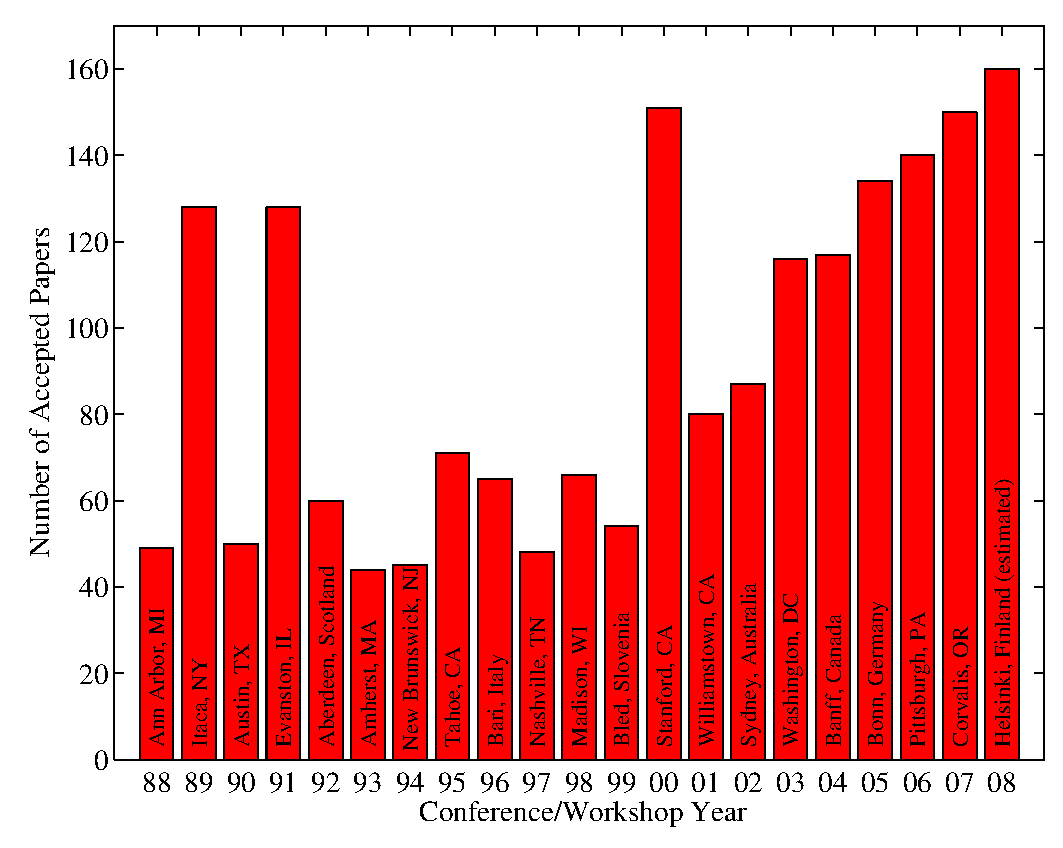
\includegraphics[width=\columnwidth]{icml_numpapers}}
\caption{Historical locations and number of accepted papers for International
Machine Learning Conferences (ICML 1993 -- ICML 2008) and International
Workshops on Machine Learning (ML 1988 -- ML 1992). At the time this figure was
produced, the number of accepted papers for ICML 2008 was unknown and instead
estimated.}
\label{icml-historical}
\end{center}
\vskip -0.2in
\end{figure}

\subsection{Figures}

You may want to include figures in the paper to illustrate
your approach and results. Such artwork should be centered,
legible, and separated from the text. Lines should be dark and at
least 0.5~points thick for purposes of reproduction, and text should
not appear on a gray background.

Label all distinct components of each figure. If the figure takes the
form of a graph, then give a name for each axis and include a legend
that briefly describes each curve. Do not include a title inside the
figure; instead, the caption should serve this function.

Number figures sequentially, placing the figure number and caption
\emph{after} the graphics, with at least 0.1~inches of space before
the caption and 0.1~inches after it, as in
Figure~\ref{icml-historical}. The figure caption should be set in
9~point type and centered unless it runs two or more lines, in which
case it should be flush left. You may float figures to the top or
bottom of a column, and you may set wide figures across both columns
(use the environment \texttt{figure*} in \LaTeX). Always place
two-column figures at the top or bottom of the page.

\subsection{Algorithms}

If you are using \LaTeX, please use the ``algorithm'' and ``algorithmic''
environments to format pseudocode. These require
the corresponding stylefiles, algorithm.sty and
algorithmic.sty, which are supplied with this package.
Algorithm~\ref{alg:example} shows an example.

\begin{algorithm}[tb]
   \caption{Bubble Sort}
   \label{alg:example}
\begin{algorithmic}
   \STATE {\bfseries Input:} data $x_i$, size $m$
   \REPEAT
   \STATE Initialize $noChange = true$.
   \FOR{$i=1$ {\bfseries to} $m-1$}
   \IF{$x_i > x_{i+1}$}
   \STATE Swap $x_i$ and $x_{i+1}$
   \STATE $noChange = false$
   \ENDIF
   \ENDFOR
   \UNTIL{$noChange$ is $true$}
\end{algorithmic}
\end{algorithm}

\subsection{Tables}

You may also want to include tables that summarize material. Like
figures, these should be centered, legible, and numbered consecutively.
However, place the title \emph{above} the table with at least
0.1~inches of space before the title and the same after it, as in
Table~\ref{sample-table}. The table title should be set in 9~point
type and centered unless it runs two or more lines, in which case it
should be flush left.

% Note use of \abovespace and \belowspace to get reasonable spacing
% above and below tabular lines.

\begin{table}[t]
\caption{Classification accuracies for naive Bayes and flexible
Bayes on various data sets.}
\label{sample-table}
\vskip 0.15in
\begin{center}
\begin{small}
\begin{sc}
\begin{tabular}{lcccr}
\toprule
Data set & Naive & Flexible & Better? \\
\midrule
Breast    & 95.9$\pm$ 0.2& 96.7$\pm$ 0.2& $\surd$ \\
Cleveland & 83.3$\pm$ 0.6& 80.0$\pm$ 0.6& $\times$\\
Glass2    & 61.9$\pm$ 1.4& 83.8$\pm$ 0.7& $\surd$ \\
Credit    & 74.8$\pm$ 0.5& 78.3$\pm$ 0.6&         \\
Horse     & 73.3$\pm$ 0.9& 69.7$\pm$ 1.0& $\times$\\
Meta      & 67.1$\pm$ 0.6& 76.5$\pm$ 0.5& $\surd$ \\
Pima      & 75.1$\pm$ 0.6& 73.9$\pm$ 0.5&         \\
Vehicle   & 44.9$\pm$ 0.6& 61.5$\pm$ 0.4& $\surd$ \\
\bottomrule
\end{tabular}
\end{sc}
\end{small}
\end{center}
\vskip -0.1in
\end{table}

Tables contain textual material, whereas figures contain graphical material.
Specify the contents of each row and column in the table's topmost
row. Again, you may float tables to a column's top or bottom, and set
wide tables across both columns. Place two-column tables at the
top or bottom of the page.

\subsection{Citations and References}

Please use APA reference format regardless of your formatter
or word processor. If you rely on the \LaTeX\/ bibliographic
facility, use \texttt{natbib.sty} and \texttt{icml2018.bst}
included in the style-file package to obtain this format.

Citations within the text should include the authors' last names and
year. If the authors' names are included in the sentence, place only
the year in parentheses, for example when referencing Arthur Samuel's
pioneering work \yrcite{Samuel59}. Otherwise place the entire
reference in parentheses with the authors and year separated by a
comma \cite{Samuel59}. List multiple references separated by
semicolons \cite{kearns89,Samuel59,mitchell80}. Use the `et~al.'
construct only for citations with three or more authors or after
listing all authors to a publication in an earlier reference \cite{MachineLearningI}.

Authors should cite their own work in the third person
in the initial version of their paper submitted for blind review.
Please refer to Section~\ref{author info} for detailed instructions on how to
cite your own papers.

Use an unnumbered first-level section heading for the references, and use a
hanging indent style, with the first line of the reference flush against the
left margin and subsequent lines indented by 10 points. The references at the
end of this document give examples for journal articles \cite{Samuel59},
conference publications \cite{langley00}, book chapters \cite{Newell81}, books
\cite{DudaHart2nd}, edited volumes \cite{MachineLearningI}, technical reports
\cite{mitchell80}, and dissertations \cite{kearns89}.

Alphabetize references by the surnames of the first authors, with
single author entries preceding multiple author entries. Order
references for the same authors by year of publication, with the
earliest first. Make sure that each reference includes all relevant
information (e.g., page numbers).

Please put some effort into making references complete, presentable, and
consistent. If using bibtex, please protect capital letters of names and
abbreviations in titles, for example, use \{B\}ayesian or \{L\}ipschitz
in your .bib file.

\subsection{Software and Data}

We strongly encourage the publication of software and data with the
camera-ready version of the paper whenever appropriate. This can be
done by including a URL in the camera-ready copy. However, do not
include URLs that reveal your institution or identity in your
submission for review. Instead, provide an anonymous URL or upload
the material as ``Supplementary Material'' into the CMT reviewing
system. Note that reviewers are not required to look at this material
when writing their review.

% Acknowledgements should only appear in the accepted version.
\section*{Acknowledgements}

\textbf{Do not} include acknowledgements in the initial version of
the paper submitted for blind review.

If a paper is accepted, the final camera-ready version can (and
probably should) include acknowledgements. In this case, please
place such acknowledgements in an unnumbered section at the
end of the paper. Typically, this will include thanks to reviewers
who gave useful comments, to colleagues who contributed to the ideas,
and to funding agencies and corporate sponsors that provided financial
support.


% In the unusual situation where you want a paper to appear in the
% references without citing it in the main text, use \nocite
\nocite{langley00}

\bibliography{example_paper}
\bibliographystyle{icml2018}


%%%%%%%%%%%%%%%%%%%%%%%%%%%%%%%%%%%%%%%%%%%%%%%%%%%%%%%%%%%%%%%%%%%%%%%%%%%%%%%
%%%%%%%%%%%%%%%%%%%%%%%%%%%%%%%%%%%%%%%%%%%%%%%%%%%%%%%%%%%%%%%%%%%%%%%%%%%%%%%
% DELETE THIS PART. DO NOT PLACE CONTENT AFTER THE REFERENCES!
%%%%%%%%%%%%%%%%%%%%%%%%%%%%%%%%%%%%%%%%%%%%%%%%%%%%%%%%%%%%%%%%%%%%%%%%%%%%%%%
%%%%%%%%%%%%%%%%%%%%%%%%%%%%%%%%%%%%%%%%%%%%%%%%%%%%%%%%%%%%%%%%%%%%%%%%%%%%%%%
\appendix
\section{Do \emph{not} have an appendix here}

\textbf{\emph{Do not put content after the references.}}
%
Put anything that you might normally include after the references in a separate
supplementary file.

We recommend that you build supplementary material in a separate document.
If you must create one PDF and cut it up, please be careful to use a tool that
doesn't alter the margins, and that doesn't aggressively rewrite the PDF file.
pdftk usually works fine. 

\textbf{Please do not use Apple's preview to cut off supplementary material.} In
previous years it has altered margins, and created headaches at the camera-ready
stage. 
%%%%%%%%%%%%%%%%%%%%%%%%%%%%%%%%%%%%%%%%%%%%%%%%%%%%%%%%%%%%%%%%%%%%%%%%%%%%%%%
%%%%%%%%%%%%%%%%%%%%%%%%%%%%%%%%%%%%%%%%%%%%%%%%%%%%%%%%%%%%%%%%%%%%%%%%%%%%%%%


\end{document}


% This document was modified from the file originally made available by
% Pat Langley and Andrea Danyluk for ICML-2K. This version was created
% by Iain Murray in 2018. It was modified from a version from Dan Roy in
% 2017, which was based on a version from Lise Getoor and Tobias
% Scheffer, which was slightly modified from the 2010 version by
% Thorsten Joachims & Johannes Fuernkranz, slightly modified from the
% 2009 version by Kiri Wagstaff and Sam Roweis's 2008 version, which is
% slightly modified from Prasad Tadepalli's 2007 version which is a
% lightly changed version of the previous year's version by Andrew
% Moore, which was in turn edited from those of Kristian Kersting and
% Codrina Lauth. Alex Smola contributed to the algorithmic style files.
